\chapter{Fundamentos Teóricos e Conceptos Previos}

O desenvolvemento dunha aplicación web non é algo trivial e mais se temos en conta todas
as peculiaridades que este proxecto contén. Para a súa comprensión é preciso coñecer unha
serie de conceptos teóricos que se expoñen a continuación:

\section{Arquitectura web}
	Neste proxecto séguese unha Arquitectura Web baseada no modelo cliente-servidor, que 
	consiste nun lado servidor que distribúe os recursos como poden ser o contido multimedia
	(vídeos, imaxes, etc) ou as páxinas web ao outro lado, o cliente, que típicamente corre 
	nun navegador web interpretando as páxinas html e o código javascript asociado a estas.
	
	No noso caso a parte servidor estará dividida en dúas compoñentes claramente diferenciadas,
	o sistema para a análise do comportamento, e a aplicación web que permitirá o acceso a este, 
	os fundamentos de ámbalas dúas partes explícanse a continuación.
	
\section{Análise do comportamento}
	É un dos campos de investigación mas activos hoxe en día. A idea principal na que se 
	centran estes sistemas como o que nos ocupa é a de detectar calquera acción levada a 
	cabo polos obxectos involucrados nunha escena de vídeo. Un obxecto é calquera cousa 
	que debe ser seguida, polo que dependendo do tipo de problema estes obxectos poden 
	ser dunha natureza ou doutra.
	O tipo de accións a detectar tamén depende da tipoloxía do sistema, xa poden ser
	comportamentos individuais( camiñar, correr, loitar...) ou grupais (reunirse, abandonar
	un grupo de persoas...).
	
	Tanto neste proxecto como nos sistemas para a análise do comportamento en xeral, 
	pódense discernir tres tarefas importantes que colaboran entre si\cite{brais-thesis}:
	
	\begin{itemize}
	
		\item{\textbf{Detección de Obxectos:}}\label{cap:DeteccionObxetos} Partindo dunha secuencia de vídeo como 
		entrada obtéñense os distintos obxectos que aparecen en cada fotograma da escena.
		Para este fin empréganse técnicas de visión por computador.
		
		%Aqui podríame extender falando da Substracción de Fondo, o Fluxo Óptico e os Sistemas de alto Nivel
		
		\item{\textbf{Seguimento de Obxectos:}} A partires da información obtida na detección, asígnanselle 
		identificadores a cada obxecto detectado no vídeo, agrupando se procede distintos
		obxectos baixo o mesmo identificador en caso de considerarse que estes obxectos forman
		parte de un grupo ou unha mesma detección.
		
		% Aquí podría falar das aproximacións por apariencia, filtro de Kalman, filtro de Partículas ..
		
		\item{\textbf{Análise do comportamento de Alto Nivel:}} Unha vez obtida a información dos 
		dous pasos anteriores pódese catalogar o comportamento de cada detección empregando
		técnicas de recoñecemento de patróns.
	
	\end{itemize}	
	
	Os resultados mais destacables destas técnicas cos que a aplicación terá que traballar serán:
	\begin{itemize}
		\item A lista de obxectos detectados para cada un dos fotogramas e a súa posición neles
		\item A traxectoria de cada un dos obxectos detectados
		\item O grao de anormalidade da traxectoria seguida por un obxecto en cada un dos fotogramas
		\item A velocidade de un obxecto determinado.
	\end{itemize}
	
	Estas tres tarefas requiren dunha serie de cálculos matemáticos baseados en técnicas moi diversas,
	para realizar toda esta serie de cálculos, empregase algunha biblioteca de código que simplifique 
	o traballo a realizar, e neste caso, esta biblioteca é OpenCV.
	
	\subsection{OpenCV}
		OpenCV é unha biblioteca libre de visión artificial escrita en código C/C++ optimizado.
		Dende a súa aparición publicada por Intel en Xaneiro de 1999, empregouse en infinidade 
		de proxectos, tanto para detección de movemento como para aplicativos de control de procesos
		que requiren recoñecemento de obxectos.
		
		OpenCV é multiplataforma, existindo versión para GNU/Linux, Mac OS X e Windows. Contén mais 
		de 500 funcións que abarcan unha ampla gama de áreas como o proceso de visión, recoñecemento
		de obxectos (tamén recoñecemento facial), calibrado de cámaras, realidade aumentada e visión
		robótica.
		
		Por todas estas características OpenCV é unha das bibliotecas mais empregadas hoxe en día, e é
		por elo tamén que se escolleu para a implementación do sistema de recoñecemento que a aplicación
		web empregará para a análise do vídeo.
		
		Non obstante, xa que se desexa que a aplicación web sexa o mais versátil posible, contemplase a
		posibilidade de que poida empregar para a análise sistemas desenvoltos noutras tecnoloxías como
		pode ser Matlab. E para dotala deste grao de versatilidade decídese definir unha interface de
		liña de comando a través da cal se chamará ao sistema, e un formato de ficheiro XML (Extensible 
		Markup Language) no que este sistema de recoñecemento deben escribir os datos da súa análise.
		
\section{Extensible Markup Language (XML)}
	XML é unha linguaxe de marcas desenvolvida polo W3C (World Wide Web Consortium) e empregado
	para almacenar datos de forma clara e lexible. Permite definir a gramática de linguaxes 
	específicas para estruturar así grandes documentos.
	
	Os documentos XML seguen una estrutura xerárquica baseada en etiquetas(tag's) e atributos,
	que se poden definir nunha Definición de Tipo de Documento ou DTD. \cite{dtd-web-page}
	
	Cando un documento en formato XML segue as directrices definidas no ficheiro DTD asociado,
	dise que este ficheiro esta ben formado(well formed en ingles), e para validar iso empregarase
	na elaboración do traballo algún avaliador de XML en liña como por exemplo o da W3Chools.\cite{xml-validator}
	
	XML é especialmente útil para comunicar varias aplicacións que traballan en tecnoloxías 
	diferentes grazas á súa simplicidade que permite integrar os datos de xeito moi sinxelo. Precisamente
	por iso, servirá como nexo de unión entre o sistema de análise que explicamos anteriormente, e a 
	aplicación web cuxos fundamentos teóricos vemos a continuación. 
	
\section{Programación Web}

	A programación web de aplicacións de carácter empresarial require do coñecemento da rede, ademais
	do de unha serie de ferramentas e estratexias para chegar a un deseño sostible e de calidade.
	
	A arquitectura clásica das aplicacións web pódese ver no gráfico \ref{fig:ArquitecturaAppWeb}
	
	\begin{figure}[htp]
	\begin{center}
		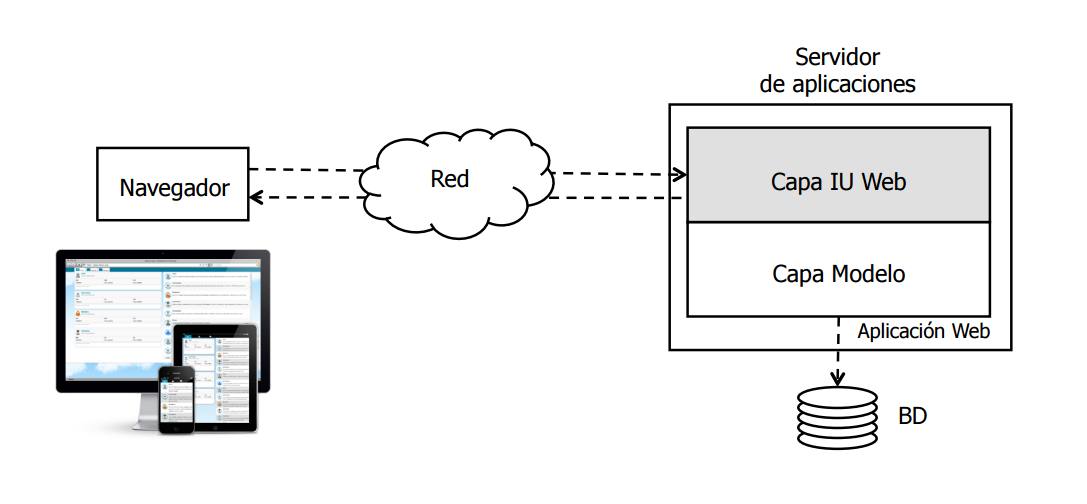
\includegraphics[scale=0.35]{figures/ArquitecturaAppWeb.png}
		\caption{Clásica arquitectura dunha aplicación web empresarial}
	\label{fig:ArquitecturaAppWeb}
	\end{center}
	\end{figure}

	As técnicas e estratexias mais importantes á hora de construír unha aplicación web relátanse nos
	puntos subseguistes:
	
	\subsection {Desenvolvemento Áxil}
		Para reducir custos e poder proporcionar solucións rápidas é preciso que as 
		aplicacións web's de caracter empresarial se leven a cabo en pouco tempo e con
		bos principios de enxeñaría, a isto contribúen en gran medida as tecnoloxías 
		que se amosan a continuación.
	
	\subsection{Soporte para transaccións}
		Unha transacción nun Sistema Xestor de Base de Datos (SGBD) é un conxunto de ordes que
		se executan formando unha unidade de traballo, de forma invisible e atómica. 
		As transaccións cobran gran importancia nas aplicacións web debido á inestabilidade 
		da rede e á concorrencia dos distintos clientes conectados, polo que é axuda a un 
		desenvolvemento moi áxil que a tecnoloxía traia a súa xestión integrada.
	
	\subsection{Object-Relational Mapping (ORM)}
		Os mapeado obxecto-relación é unha das técnicas de programación que mais velocidade imprimen
		na construcción de webs, xa que converte os datos dunha linguaxe Orientada a Obxectos (OO) a 
		datos de un sistema relacional no que son persistidos e viceversa, aforrando ao programador
		o traballo de ter que programar o código para esta tarefa. É desexable pois que a tecnoloxía
		a empregar dispoña de un mapeador obxecto-relacional ben integrado, algúns exemplos disto poden
		ser: a combinación Java+Maven+Hibernate, o EF(Entity Framework) de Microsoft ou os Models de Django.
	
	\subsection{Xestión de Layout}
		Tamén resulta moi practico dispoñer dunha linguaxe de prantilla que permitan xerar contido
		html ben estruturado dinamicamente. Algúns exemplos son o Sistema de Templates de Django, o 
		Sistema JSP de Spring, a libraría Thymeleaf ou os compoñentes de ASP.NET. Todos eles axudan 
		a xerar contido HTML de xeito sinxelo e escalable.
		
	\subsection{Outras cuestións da web}
		A maiores existe toda unha gama de outras funcionalidades que cobran importancia cando deseñamos
		e construímos unha web como o manexo de erros nos formularios, internacionalización (i18n), 
		visualización de grande cantidades de datos(en listas ou táboas), seguridade...
		
		
\section{O Vídeo}

    \subsection{Formato de Vídeo}
    
    \subsection{Codec's}

    \subsection{Streaming de Vídeo}
        Dado que este proxecto está centrado no tratamento de vídeo, é de especial importancia ver 
        de que xeitos podemos distribuílo e reproducilo a través da rede. A estes efectos existen dúas
        grandes alternativas que varían en canto ao seu grao de escalabilidade, dificultade de 
        implementación, e calidade final do servizo:
        
        \subsection{Pseudo Streaming ou Descarga Progresiva}
            Consiste na descarga do vídeo por fragmentos, típicamente empregando o protocolo HTTP. 
            Neste formato, o reprodutor vai acumulando fragmentos de vídeo ata obter os precisos como 
            para comezar a reprodución, mais se o ancho de banda fose insuficiente, o vídeo remataría
            por pararse. Este sistema é o empregado por servizos como YouTube, Vimeo, DailyMotion...
            
            Será a opción empregada por motivos de simplicidade, mais compre explicar tamén o verdadeiro 
            Streaming, xa que é a diferenza do pseudo-streaming pode ser empregado para a emisión de
            contido en directo como o dunha cámara de seguridade.
            
        \subsection{Streaming}
            O verdadeiro streaming ( do inglés True Streaming) consiste na emisión en directo do 
            contido multimedia a través da rede, que o reprodutor reproduce no momento que recibe.
            Este outro xeito de distribuír vídeo, apoiase en axustar a calidade do vídeo ao ancho de
            banda do que dispón o cliente, evitando así interrupcións na reprodución.
            
            O protocolo mais destacable á hora de empregar este tipo de streaming é RTSP (Real-Time
            Streaming Protocol) que operando a nivel de aplicación permite controlar un ou varios fluxos 
            sincronizados de contido multimedia.
            
            Por unha parte RTSP soe empregar o Real-Time Transport Protocol (RTP) sobre UDP(User 
            Datagram Protocol) para o transporte de contido multimedia, maximizando así o emprego 
            da rede pero sen garantir un mínimo na calidade do servizo.
            
            E por outra parte RTSP emprega o Real-time Control Protocol (RTCP) sobre TCP(Transmission 
            Control Protocol) para a transmisión periódica de paquetes de control da sesión, o
            diagnóstico de fallos e o control de la calidade da transmisión.
            
            \begin{figure}[htp]
            \begin{center}
                
\includegraphics[scale=0.6]{figures/RTPS-diagram.png}
                \caption{Diagrama conexión RTPS}
            \label{fig:RTPS-diagram}
            \end{center}
            \end{figure}
            
            RTSP asemellase a HTTP no formato das peticións/repostas e na sintaxe, pero dispoñendo 
            dun estado que permite tanto a clientes como a servidores facer peticións.

            Tamén existen outros protocolos propietarios como MMS (Microsoft Media Server)ou RTMP 
            (Real-Time Messaging Protocol) e RTMFP (Real-Time Media Flow Protocol) de Adobe.
  
\chapter{Análise de antecedentes e alternativas}
	Se trata de realizar un estudio de alternativas o “estado del arte” o un análisis comparativo
	de alternativas.

	Se exponen las diferentes alternativas que se han evaluado o que se consideran de interés, a
	lo realizado en el proyecto. Fundamentalmente se trata de otras herramientas existentes 
	que realizan algo similar, sean o no comerciales, o de prototipos de investigación relacionados,
	o de estudios que tratan aspectos similares.

	Buscar por internet produtos que fagan algo similar...